\documentclass[letter,11pt]{article}
\usepackage[letterpaper,text={6.5in,9in}]{geometry}

%%%%%%% additions for space %%%%%%%%%%
\usepackage{setspace}
%\renewcommand{\topfraction}{0.85}
%\renewcommand{\textfraction}{0.1}
%\renewcommand{\floatpagefraction}{0.75}
%\setstretch{0.96}
%%%%%%%%%%%%%%%%%%%%%%%%%%%%%%%%%%%%%%
\usepackage{float}
\usepackage{authblk}
\usepackage{hyperref}
\usepackage{amsfonts}
\usepackage{amsmath}
\usepackage{amssymb}
\usepackage{amsthm}
\usepackage{graphicx}
\usepackage{color}
\usepackage[none]{hyphenat}
\usepackage{wrapfig}
\usepackage[justification=centering]{caption}
\usepackage{bm}
\usepackage{enumitem}
\usepackage{bbm}
\usepackage{subcaption}
\usepackage[makeroom]{cancel}
\usepackage{amsmath}
\usepackage{caption}
\usepackage{array}
\usepackage{listings}

\theoremstyle{plain}
\newtheorem{theorem}{Theorem}[section]
\newtheorem{lemma}[theorem]{Lemma}
\newtheorem*{claim}{Claim}
\newtheorem{corollary}[theorem]{Corollary}
\theoremstyle{definition}
\newtheorem{definition}[theorem]{Definition}
\newtheorem{observation}[theorem]{Observation}
\newtheorem*{remark}{Remark}
\usepackage{graphicx}
\usepackage{subcaption}
\usepackage{algorithm}
\usepackage[noend]{algpseudocode}

\theoremstyle{plain}
\theoremstyle{definition}

\graphicspath{ {Figures/} }

\newcommand{\Xomit}[1]{}
\newcommand{\fix}[1]{\textbf{\textcolor{red}{#1}}}
\newcommand{\new}[1]{\textcolor{cyan}{#1}}

\begin{document}
	
	\pagenumbering{gobble}
	\begin{titlepage} % Suppresses displaying the page number on the title page and the subsequent page counts as page 1
		\newcommand{\HRule}{\rule{\linewidth}{0.5mm}} % Defines a new command for horizontal lines, change thickness here
		
		\center % Centre everything on the page
		
		%------------------------------------------------
		%	Headings
		%------------------------------------------------
		\textsc{\LARGE Tel Aviv University}\\[1.5cm] % Main heading such as the name of your university/college
		\textsc{\Large Deep Learning Course}\\[0.5cm] % Major heading such as course name
		\textsc{\large Project Report}\\[0.5cm] % Minor heading such as course title
		
		%------------------------------------------------
		%	Title
		%------------------------------------------------
		\HRule\\[0.4cm]
		{\LARGE\bfseries Universal Style Transfer via Feature Transforms}\\[0.4cm] % Title of your document (huge)
		\HRule\\[1.5cm]
		
		%------------------------------------------------
		%	Author(s)
		%------------------------------------------------
		{\large\textit{Authors}}\\
		\begin{center}
			\begin{tabular}{c c}
				Eyal \textsc{Waserman} & Carmi \textsc{Shimon}\\% Your name
				305210189 & 201627320 \\
				waserman.eyal@gmail.com & carmishimon1@gmail.com
			\end{tabular}
		\end{center}
		
		%------------------------------------------------
		%	Date
		%------------------------------------------------
		
		\vfill\vfill\vfill % Position the date 3/4 down the remaining page
		{\large\today} % Date, change the \today to a set date if you want to be precise
		
		%------------------------------------------------
		%	Logo
		%------------------------------------------------
		%\vfill\vfill
		%\includegraphics[width=0.2\textwidth]{placeholder.jpg}\\[1cm] % Include a department/university logo - this will require the graphicx package
		
		%----------------------------------------------------------------------------------------
		\vfill % Push the date up 1/4 of the remaining page
		
	\end{titlepage}
	\pagenumbering{arabic}
	

	%\section{Abstract}
	\label{abs_lbl}
	\begin{abstract}
Style transfer is a technique of recomposing a content image with the artistic style of another. In this project, we implement an algorithm for \textit{Universal} Style Transfer, which means it is not limited to predefined styles. This is done through Feature Transforms of whitening and coloring. Using feature extractors and inverters, we are able to apply these transforms to deep features of the content image in order to match their statistics to those of the style image. This covariance matching essentially transfers the style while preserving the content, so the image reconstructed by the feature inverter is a style transferred image. Our implementation serves as a PyTorch tool ready to be used by users and researchers. Moreover, we offer an innovative approach to enhance the style transfer effect, and other approaches to transfer style from a pair of style images more efficiently than before.
\end{abstract}
%	Style transfer is the technique of recomposing images in the style of other images.
%Universal style transfer aims to transfer arbitrary visual styles to content images.
%Existing feed-forward based techniques would need to be trained on pre-defined styles and then fine tuned for new styles. Whereas, this paper presents new methods which are completely independent of the style during train phase making it a “learning-free” approach.
%In this paper, we present an encoder-decoder architecture where the encoder serves as feature-extractor and the decoder is trained for image reconstruction. 
%The Goal is to build a new Image which has the contents of the Content Image and style of the Style Image.
%Our results provide new insights handling arbitrary styles in an efficient-Learning-free methods.
	
	\section{Introduction}
	\label{intro_lbl}
	% What is style transfer?
\hspace{0.5cm} Style transfer (ST) is an image editing task, which given two examples, aims to synthesize a new image in a way that preserves the \textit{content} of one and the \textit{artistic style} of the other. Since many ST algorithms are trained to deal with predefined styles, an algorithm that works in a style agnostic manner is called Universal Style Transfer.
% What is in the UST paper?
In their paper "Universal Style Transfer via Feature Transforms" (NIPS 2017) \cite{bib11}, Li et al. show how the feature representations learned by high-performing CNNs (Encoder) followed by efficient feature Whitening-Coloring transforms (WCTs) and a compatible reconstruction (Decoder) can be used to perform the ST task. In their algorithm, which we refer to as UST throughout this paper, the two key building blocks are the encoder-decoder pairs and the WCT transform. The encoders are VGG based CNN feature extractors. Every such encoder has a matching decoder with symmetric architecture to perform image-reconstruction through feature-inversion. The style transfer process is conducted by transforming the content features at intermediate layers according to the statistics of the style features. This transformation takes place right after feature extraction (encoder) and before image reconstruction (decoder). Li et al. found that the classical signal whitening and coloring transforms are very efficient to this purpose.\\
% What are out results and innvoations?
In this project we implemented the UST algorithm in PyTorch. The goal for this implementation is to be a useful Style Transfer CLI tool. It is ready for use once downloaded from our GitHub: \url{https://github.com/eyalw711/universal_style_transfer}. Additionally, since it is designed to have lighter code volume than existing implementations, and offers more control, it should also appeal to researchers wanting to study various aspects of UST. Furthermore, in this project we trained decoder models for image reconstructions and experimented with sequentially and separately training each network block at a time. For this part we offer insight as to the time and resources it takes to train these models. Finally, as part of the project, we conducted two studies for methods to improve the UST algorithm, and both of which yielded results. In the first study, we looked at methods to synthetically increase the number channels in the feature representation of the input images, hoping to gain a stronger style transfer effect. This study yielded the innovative \textit{Boost} step, which we demonstrate to yield results with finer details and richer colors. The other study focused on new, efficient ways to transfer style from two style images at once. This study yielded three new techniques to perform this task, all of which are computationally more efficient than the one proposed in \cite{bib11} while demonstrated to have on-par results. \\

Our main contributions and results:
\begin{itemize}
	\item PyTorch Tool ready to be used by users to perform style transfer, and by researchers in order to study new models, methods or use-cases for UST.
	\item We present innovative approach to enhance the style transfer effect and demonstrate its effectiveness in producing visually pleasing results featuring more details and colors.
	\item We present new efficient techniques to perform ST from two style images at once. We show that these techniques produce visually pleasing results while using less computational resources thus saving runtime. 
\end{itemize}

%In this project, we implement the UST algorithm as a PyTorch Tool both ready to be used by users to perform style transfer, and to be used by researchers in order to study new models, methods or use-cases for UST.
%We introduce a novel methods which boosts style transfer by taking advantage of the existence of feature representations from state-of-the-art CNNs.  
%We also show new and efficient methods of combining different style images into the target image (content image) by using WCT algorithm efficiently.
%Our goal was to invent new and efficient ways of UST based on the work by Li et al. \cite{bib11}.
%Our method consists of a stylization step and a smoothing step. Both have a closed-form solution and can be computed efficiently. The stylization step is based on the (WCT) \cite{bib10}, which stylizes images via feature projections. The WCT was designed for artistic stylization.
%Our results show similar results as presented in \cite{bib10} while showing efficiency in computation.\\


% sentence pool
%The key challenge is how to extract effective representations of the style and then match it in the content image.
%Transferring the style from one image onto another can be considered a problem of texture transfer. In texture transfer the goal is to synthesize a texture from a source image while constraining the texture synthesis in order to preserve the semantic content of a target image. For texture synthesis there exist a large range of powerful non-parametric algorithms that can synthesise photo realistic natural textures by re-sampling the pixels of a given source texture \cite{bib1, bib2, bib3, bib4}. Most previous texture transfer algorithms rely on these non-parametric methods for texture synthesis while using different ways to preserve the structure of the target image. For instance, Efros and Freeman introduce a correspondence map that includes features of the target image such as image intensity to constrain the texture synthesis procedure \cite{bib3}. Lee et al. improve this algorithm by additionally informing the texture transfer with edge orientation information \cite{bib5}. Although these algorithms achieve remarkable results, they all suffer from the same fundamental limitation: they use only low-level image features of the target image to inform the texture transfer. Ideally, however, a style transfer algorithm should be able to extract the semantic image content (e.g. the objects and the general scenery) and then inform a texture transfer procedure to render the semantic content of the target image (content and style image) in the style of the style image. Therefore, a fundamental prerequisite is to find image representations that independently model variations in the semantic image content and the style in which it is presented.
%To generally separate content from style in natural images is still an extremely difficult problem.\newline
%However, the recent advance of Deep Convolutional Neural Networks (CNNs) \cite{bib6} has produced powerful computer vision systems that learn to extract high-level semantic information from natural images.  It was shown that CNNs trained with sufficient labeled data on specific tasks such as object recognition learn to extract high-level image content in generic feature representations that generalize across data sets \cite{bib7} and even to other visual information processing tasks, including texture recognition \cite{bib8} and artistic style classification \cite{bib15}.\newline
%The main issue is how to properly and effectively apply the extracted style characteristics (feature correlations) to content images in a style-agnostic manner.\newline


	
	\section{Related Work}
	\label{related_lbl}
	\hspace{0.5cm} Existing stylization methods can be classified into two categories: global and local. Global methods \cite{bib12, bib13} achieve stylization through matching the means and variances of pixel colors \cite{bib12}. Local methods \cite{bib14} stylize images through finding dense correspondences between the content and style photos based on either low-level or high-level features. These approaches are slow in practice. Also, they are often developed for specific scenarios. Therefore these methods do not scale to the setting of arbitrary style images well. Gatys et al. \cite{bib7, bib8} showed remarkable results by using the VGG-19 deep neural network for style transfer. The major step in the algorithm is to solve an optimization problem of matching the Gram matrices of deep features extracted from the content and style images. A number of methods have been developed \cite{bib15, bib16, bib17} to further improve its stylization performance and speed. However, these methods do not aim to preserve photorealism. Their approach was taken up by various follow-up papers that, among other things, proposed different  ways  to  represent  the  style  within  the  neural  network. Li et al. \cite{bib15} suggested an approach to preserve local patterns of the style image. Instead of using a global representation of the style, computed as Gram matrix. Nikulin et al. \cite{bib18} tried the style transfer algorithm by Gatys et al. on other nets than VGG and proposed several variations in the way the style of the image is represented  to archive different goals like illumination or season transfer. However, this method is developed for specific scenarios which cannot be scaled to the setting of arbitrary style images. This project is an extension of UST \cite{bib11}, which is closest to a related work \cite{bib19}, directly adjusts the content feature to match the mean and variance of the style feature. However, the generalization ability of the learned models on unseen styles is still limited. UST is also closely related to \cite{bib15}, where content feature in a particular (higher) layer is adaptively instance normalized by the mean and variance of style feature. This step can be viewed as a sub-optimal approximation of the WCT operation, thereby leading to less effective results on both training and unseen styles. Moreover, the  encoder-decoder network in \cite{bib11} is trained solely based on image reconstruction, while \cite{bib15} requires learning such a module particularly for stylization task. Different from the existing methods, the approach in \cite{bib11} is to perform style transfer efficiently in a feed-forward manner while achieving generalization and visual quality on arbitrary styles. 
	
	\section{Methods}
	\label{methods_lbl}
	\hspace{0.5cm} This project deals with the paper of Universal Style Transfer via Feature Transforms \cite{bib11}. Its main goals are to implement the proposed algorithm in PyTorch, and to add innovations in its capabilities. The code for our implementation is in the repository \url{https://github.com/eyalw711/universal_style_transfer}. Our innovations include a new \textit{boosting} technique to enhance the style transfer effect, and three new merging to techniques to transfer style from two images simultaneously. This section describes the methods in which we tackled the following tasks: 
\begin{itemize}
	\item Building and training the models required for Universal Style Transfer via Feature Transforms as described in \cite{bib11}.
	\item Implementing a PyTorch program to perform the UST algorithm as described in \cite{bib11}.
	\item Present innovative method to enhance the style transfer effect. This method shall be referred to as \textit{Boosting}.
	\item In \cite{bib11}, Li et al. present a method to transfer style from a pair of style images, in such a way that the result will contain stylistic aspects of both. Let's refer to this problem as \textit{Merge}-UST. In this task we research methods that utilize the UST framework to perform Merge-UST in a computationally lighter fashion than the original.
\end{itemize}


\subsection{Models and Training}\label{subsec:Models}
\label{models_methods_lbl}
\hspace{0.5cm} In their paper \cite{bib11}, Li et al. describe that in order to perform UST, the models required are five pairs of encoder-decoders trained only for image reconstruction (and not for style transfer). The importance of this is that the models never see style images during their training, which leads to their ability to generalize to unlimited number of styles once fully trained, achieving the \textit{universal} in UST. Li et al. used models based on the VGG-19 CNN feature extractor architecture. These networks work as a pipeline where each encoder-decoder pair is a level (see Fig.~\ref{fig:full-pipeline}). In each such level, the encoder serves as feature extractor while the decoder does the inverse operation, reconstructs the image from the extracted features.\\
We based our solution on the implementation of VGG-19 \cite{bib20} from \texttt{torchvision.models} which is trained for image classification on the ImageNet dataset (Deng et al.) \cite{bib21}. The model is available with pretrained weights. Its CNN feature extractor has the following architecture:
\begin{gather*}
[64, 64, MP, 128, 128, MP, 256, 256, 256, 256, MP, 512, 512, 512, 512, MP, 512, 512, 512, 512, MP]
\end{gather*}
Any numeric $d$ entry indicates a 2D-convolution layer with $d$ output channels, and MP entries indicate MaxPool layers.

\subsubsection{Encoders}\label{subsec:Encoders}
In order to build the five encoders, we load the \texttt{torchvision.models} VGG-19 pretrained model and trim it in the following way:
\begin{itemize}
	\item Encoder-1: [64]
	\item Encoder-2: [64, 64, MP, 128]
	\item Encoder-3: [64, 64, MP, 128, MP, 256]
	\item Encoder-4: [64, 64, MP, 128, MP, 256, 256, 256, 256, MP, 512]
	\item Encoder-5: [64, 64, MP, 128, MP, 256, 256, 256, 256, MP, 512, 512, 512, 512, MP, 512]
\end{itemize}
The encoders are initialized with pretrained weights and thus the project does not include encoder training. For next sections, denote Encoder-$j$ as $E_j$.

\subsubsection{Decoders}\label{subsec:Decoders}
The architecture of the decoders is generally inverse to that of the encoders, in order to achieve image-reconstruction. We defined five decoder \textit{blocks} the following way:
\begin{itemize}
	\item Decoder-Block-1: (64)[3]
	\item Decoder-Block-2: (128)[64, US, 64]
	\item Decoder-Block-3: (256)[128, US, 128]
	\item Decoder-Block-4: (512)[256, US, 256, 256, 256]
	\item Decoder-Block-5: (512)[512, US, 512, 512, 512]
\end{itemize}
The number in parenthesis in each row stands for the number of input channels for the block, and every 'US' entry stands for an Up Sampling layer. Let's denote Decoder-Block-$j$ by $B_j$. Each decoder then is built as such:
\begin{equation}\label{eq:decoder}
D_j(x) = B_1 \circ \dots \circ B_j (x)
\end{equation}
Notice that $D_j(E_j(x))$ yields $\hat{x}$ with the same size as $x$.\\

Decoder training was done with two steps: Decoder-Block sequential training, followed by Fine-Tune phase.
\begin{itemize}
	\item \textbf{Decoder-Block sequential training}: Initially $B_1$ was trained to reconstruct images encoded by $E_1$. Afterwards, each $B_j, j>1$ was trained once all $j-1,\dots,1$ had finished training to some reasonable degree. In training $B_j$, the reconstruction result for image $x$ was calculated by:
	\begin{gather*}
	\hat{x} = D_{j-1} \circ B_j \circ E_j (x)
	\end{gather*}
	In this calculation all functions except $B_j$ are fixed. Since $B_{j-1}, \dots, B_1$ are already pretrained to some degree when training $B_j$, then $B_j$ learns to transform $E_j$'s output to $D_{j-1}$ input. The sequential blocks training is implemented in the \texttt{train\_block} function in \texttt{seq\_models.py} file. Use '\texttt{python seq\_models.py -h}' for help.\\
	This step is important since the deeper the architecture of the decoder goes, the larger the models are, and the slower the weights converge in training. Having to train only a part of the model at first (where the rest is already trained) removes degrees of freedom, and assures it converges faster to a reasonable degree. Also, whenever all 5 blocks are trained, they serve as a good starting point for the next stage.

	\item \textbf{Fine-Tune Phase}: Each decoder $D_j$ is built according to Equation~\ref*{eq:decoder} with the pretrained blocks acquired in the previous step. With none of the blocks frozen, the entire $D_j$ is now trained for image reconstruction against $E_j$ and ultimately is saved as a decoder (and not as a bundle of blocks). The fine-tune training is implemented in the \texttt{train\_decoder} function in \texttt{models\_utils.py} file. Use '\texttt{python models\_utils.py -h}' for help.
\end{itemize}

Throughout this section, the loss function for training the models is:
\begin{equation}\label{eq:loss}
L = MSE(I_o-I_i) + \lambda \cdot MSE(\Phi(I_o)-\Phi(I_i))
\end{equation}
$\lambda$ was set to $1.0$ during training as advised by Li et al. in their paper \cite{bib11}. This loss function is derived from Equation 1 at \cite{bib11}, with the difference that we use $MSE$ where Li et al. use $L2 -loss$. We chose to use $MSE$ since different encoders $\Phi$ extract different dimensions features, causing the $L2$ loss to be somewhat not as normalized as the $MSE$. For example, an input image $I_i$ of dimensions [3,1024,1024] would have features $f_4=E_4(I_i)$ of dimension [512, 128, 128], 8,388,608 total entries, whereas it would have $f_5=E_5(I_i)$ of dimension [512, 64, 64], 2,097,152 total entries. In this example, the dimension difference causes the feature loss to be much more important in $D_4$ training than in $D_5$ under $L2$, while we believe it shouldn't.\\

When training $D_4, D_5$ we encountered a problem where every region with a "texture" such as tree leaves or sand in the original image would be translated into "boxy" artifacts in the reconstructed image. This is often an issue encountered in deep CNNs and to solve it we set the UpSampling in blocks 4,5 to "bilinear" whereas originally we tried training all blocks with "nearest" UpSampling. Another issue we had was when training $D_1$, which performs one convolution only. Its outputs showed clear border artifacts. To mitigate them we set the padding method of $B_1$ from zero-padding to replicate-padding in $D_1$ only.\\

The dataset on which the models were trained is the COCO Dataset, a large-scale object detection, segmentation, and captioning dataset. The dataset, on top of the images it contains, offer numerous annotations such as image segmentation and classification data. We trained the models on the "test" and "validation" sets only. These sets combined contain 25k images. The annotations were unused in the training process since the decoder only trains for image reconstruction.

\subsection{UST Algorithm}
\label{algo_methods_lbl}
The UST algorithm as described in \cite{bib11} formulates style transfer as an image reconstruction process coupled with feature transformation of whitening and coloring (WCT). The reconstruction step is responsible for inverting features back to the RGB space, the feature transformation step matches the feature statistics of a content image to a style image. The file \texttt{universal\_style\_transfer.py} implements the UST algorithm, use '\texttt{python universal\_style\_transfer.py -h}' for help.

\subsubsection{Architecture}\label{subsec:arch}
The basic building block of the UST is a pair of VGG based encoder and decoder, explained and described in section ~\ref{models_methods_lbl}. A single level stylization pass in UST would be to pass a content image and a style image through an encoder, perform a transformation called WCT on the extracted content features, and then to reconstruct the output of the WCT using the decoder. The image output by the decoder should have both the original content and some notion of the artistic styles in the style image.\\ To achieve better results, UST does more than a single level stylization pass, it constructs a pipeline of such levels, each with its own encoder-decoder pair. Passing the content through this pipeline transfers style in different feature depths, so the result is generally more pleasing. See figure ~\ref{fig:full-pipeline} for a block diagram of the pipeline pass to perform UST on a pair of images $c,s$. In the following sections, for the $j$-th level of the pipeline denote the encoder by $E_j$ and the decoder by $D_j$.

\begin{figure}[h!]
	\centering
	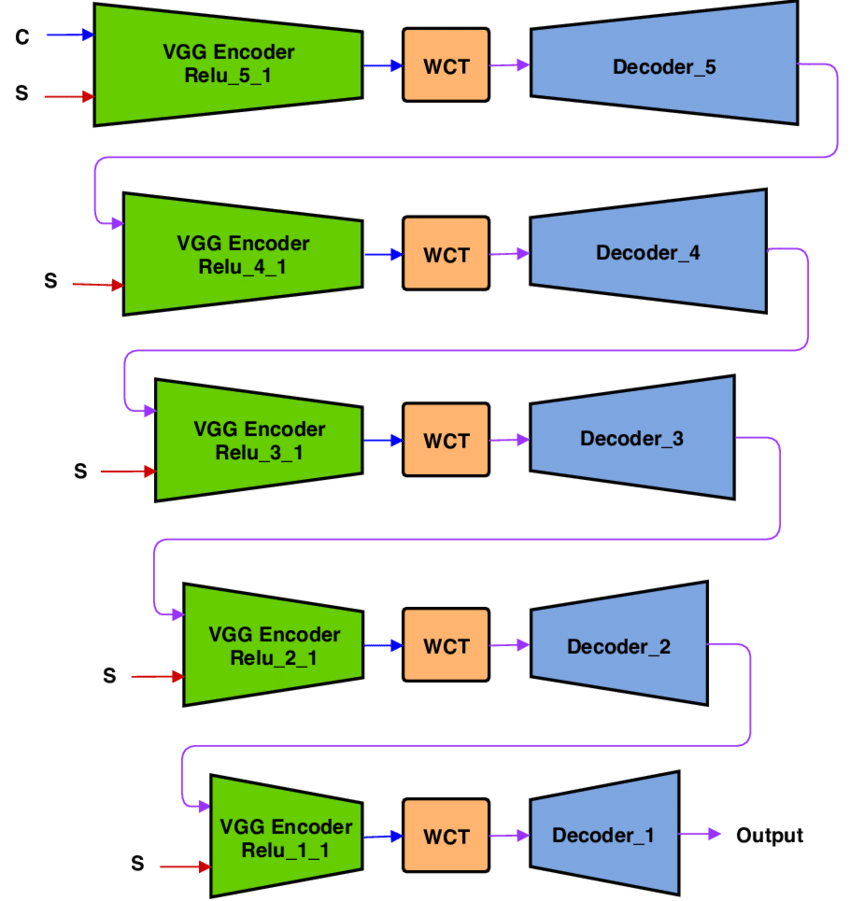
\includegraphics[width=0.5\linewidth]{UST_arc_mlt_level_pipeline.png}
	\caption{Universal Style Transfer pipeline architecture. Each level of stylization consists of single encoder-WCT-decoder network with different decreasing number of VGG layers. C and S are content and style images, respectively.
	}
	\label{fig:full-pipeline}
\end{figure}

\subsubsection{WCT} As explained above, given a pair of content image $I_C$ and style image $I_S$ as input for the $j$-th level, at first the encoder extracts their features by $f_c = E_j(I_C)$, $f_s = E_j(I_S)$. Notice that these features are three dimensional, $f_c$ is $[c\times h \times w]$ and $f_s$ is $[c\times h' \times w']$. Their height and width are generally different but their number of channels, $c$, is the same.\\
The WCT is a pair of projection functions working on vectorized VGG features. The term \textit{vectorized} means that we treat every channel of the feature tensor as a row vector, so $\vec{f_c}$ is $[c \times hw]$ and $\vec{f_s}$ is $[c \times h'w']$. WCT works on the features extracted by the encoder, and its result is fed to the decoder, as seen in Figure ~\ref{fig:full-pipeline}. WCT is a composition of a whitening transform ($\hat{f}_C$) and a coloring transform ($\hat{f}_{CS}$). The key idea behind the WCT is to directly match feature correlations of the content image to those of the style image via those two projections. Specifically, the WCT transform is applied to the vectorized content and style feature $\vec{f_c}$, $\vec{f_s}$ respectively via:\\
%%%%%%%%%%%%%%%%%%whitening%%%%%%%%%%%%%%%%%%%%%%
\textbf{Whitening:}\\
\begin{equation}
Centered\_\vec{f_c} = \vec{f_c} - mean(\vec{f_c})
\end{equation}
\begin{equation}
\hat{f_c}\hat{f_c}^T=I \Rightarrow  \hat{f_c} = E_cD_c^{-\frac{1}{2}}E_c^TCentered\_\vec{f_c} 
\end{equation}
Where $D_c$ is a diagonal matrix with the eigenvalues of the covariance matrix $Centered\_\vec{f_c}Centered\_\vec{f_c}^T=E_cD_cE_c^T \in\mathbb{R}^{cxc}$, and $E_c$ is the corresponding orthogonal matrix of eigenvectors, (see figure ~\ref{fig:WCT-vis} (a)). Both matrices obtained by using Singular Value Decomposition (SVD).\\
%%%%%%%%%%%%%%%%%%coloring%%%%%%%%%%%%%%%%%%%%%%
\newline\textbf{Coloring:}\\
Coloring transform is the inverse of the whitening transform, see figure ~\ref{fig:WCT-vis} (b)).
\begin{equation}
Centered\_\vec{f_s} = \vec{f_s} - mean(\vec{f_s})
\end{equation}
\begin{equation}
\hat{f_{cs}}\hat{f_{cs}}^T=f_sf_s^T \Rightarrow  \hat{f_{cs}} = E_sD_s^{\frac{1}{2}}E_s^TCentered\_\vec{f_c} 
\end{equation}
Where $D_s$ is a diagonal matrix with the eigenvalues of the covariance matrix $Centered\_\vec{f_s}Centered\_\vec{f_s}^T \in\mathbb{R}^{cxc}$, and $E_s$ is the corresponding orthogonal matrix of eigenvectors, both matrices also obtaind by SVD.\\
Now, we add the mean vector of the style:
\begin{equation}
\hat{f_{cs}} = \hat{f_{cs}}+mean(\vec{f_s})
\end{equation}

After the transformation, the correlations of transformed content features match those of the style, i.e., $\hat{f_{cs}} \hat{f_{cs}}^T = \vec{f_s} \vec{f_s}^T$.
The WCT performs well for artistic image stylization. However it generates
structural artifacts (e.g., distortions on object boundaries)
WCT is implemented in the function \texttt{wct} in file \texttt{utils.py}.

\begin{figure}[h!]
	\centering
	\begin{subfigure}[b]{0.4\linewidth}
		\includegraphics[width=\linewidth]{whitening.png}
		\caption{Data whitening}
	\end{subfigure}
	\begin{subfigure}[b]{0.4\linewidth}
		\includegraphics[width=\linewidth]{coloring.png}
		\caption{Data coloring}
	\end{subfigure}
	\caption{Whitening-Coloring-Transformation}
	\label{fig:WCT-vis}
\end{figure}

\subsubsection{Texture Synthesis}\label{subsec:texture}
UST has application as universal texture synthesizer too. To conduct texture synthesis, simply perform UST while setting the content image as a random noise image. The evaluation criterion for the quality of the synthesized texture is usually human inspection and textures are successfully synthesized if a human observer cannot tell the original texture from a synthesized one.

\subsection{Boost}
\label{boost_methods_lbl}
The Boost step is a fruit of our invention, and it enhances the effect of style transferral of the UST in selected regions of the image. The motivation for this \textbf{boosting} method comes from the desire to better utilize the capability to perform a constant number of SVD calls on matrices as big as $[512\times 512]$ without slowing down UST considerably. The time complexity of SVD is $O(n^3)$ for square matrices, so we treat 512 as the upper bound on the size of matrices we want to call SVD on. Empirically, SVD works in reasonable time on square matrices up to the upper bound, but we expect its runtime to grow rapidly for larger matrices. In the pipeline described in Figure ~\ref{fig:full-pipeline}, levels 1 and 2 use $E_5, E_4$ respectively to extract a 512-channels feature map representation of $I_c$ and $I_s$. This leads the WCT procedure to make two SVD calls on $[512\times 512]$ matrices, as described in ~\ref{subsec:arch}. We consider these calls \textit{efficient}. On the contrary, in levels 3,4,5, the encoders extract feature maps with 256, 128 and 64 channels respectively. These calls are \textit{inefficient} since they call SVD on matrices of size lower than the upper bound.\\

The \textit{Boost} step is a procedure done after the WCT had output $f_{cs}$ and before image reconstruction took place, in levels of the pipeline where there are inefficient SVD calls, i.e. in architectures 1, 2 and 3. At encoder-decoder architecture $j\in\{1,2,3\}$, let $x$ be the input content, $f_c = E_j(x)$ be the content features of dimensions $[c \times h \times w]$, and $f_s = E_j(s)$ be the style image features of dimensions $[c \times h' \times w']$. The number of channels $c$ is either 64, 128 or 256. The \textit{Boost} step consists of the following sub-steps:
\begin{enumerate}
	\item This sub-step will synthetically create $f_c^b$ and $f_s^b$ of 512 channels with reduced height and width, such that the total number of entries in $f_c$ is the same as in $f_c^b$ and likewise for $f_s$ and $f_s^b$. Maintaining tensor sizes is important since many times regular UST is working close to the GPU memory limit also without boosting, so we wouldn't wish to create tensors much larger than we already handle. For architecture-1, $c=64$. Choose 8 rectangular regions of size $[c \times h/4 \times w/2]$ from $f_c$ and 8 rectangular regions of size $[c \times h'/4 \times w'/2]$ from $f_s$. The regions are to be stacked on the channel dimension to achieve $f_c^b$ of size $[8c \times h/4 \times w/2]$ and $f_s^b$ of size $[8c \times h'/4 \times w'/2]$. Notice that $8c=512$ as desired. Similarly for architecture-2, choose 4 regions while dividing both height and width by factor of 2. For architecture-3 choose 2 regions while dividing height by 2, width is not divided in this case. Parts (a), (b) and (c) in Figure ~\ref{fig:boost} depict this sub-step. 
	
	\item Call the WCT procedure on $f_c^b$ and $f_s^b$ to obtain $f_{cs}^b$. Since both $f_c^b$ and $f_s^b$ have 512 channels, the two SVD calls in the WCT decompose $[512\times 512]$ matrices. Depicted in part (d) of Figure ~\ref{fig:boost}.
	
	\item Next, split $f_{cs}^b$ across the channel dimension to invert the stacking operation done previously. Let these splits be $r_1^b, \dots r_d^b$ where $d\in\{2,4,8\}$ depending on the architecture. These splits are now being treated as boosted style transformed regions of $f_{cs}$. For architecture-1 we get 8 such regions, for arch-2 we get 4 and for arch-3 we get 2.
	
	\item Lastly, blend these regions with $f_{cs}$. Let $R_i$ be the indices slicing region $i$ from $f_c$, i.e. $f_c[R_i]$ is the $i$-th region, then:
	\begin{equation}
	f_{cs}[R_i] = (1-k)\cdot f_{cs}[R_i] + k\cdot r_i
	\end{equation}
	$k$ is a kernel the size of the regions $r_i$ that diminishes close to its exterior. Its purpose is to blend $r_i$ into $f_{cs}[R_i]$ with no visible border artifacts. For $k$ we used a 2D raised-cosine which answers this requirement. See implementation in \texttt{raised\_cosine\_kern} function in \texttt{utils.py} file. The last two sub-steps are depicted in part (e) of Figure ~\ref{fig:boost}.
\end{enumerate}
The boost step is implemented in \texttt{boost} function in \texttt{utils.py}. It can be used by adding the argument \texttt{--boost} when running \texttt{universal\_style\_transfer.py}\\

\begin{figure}[h!]
	\centering
	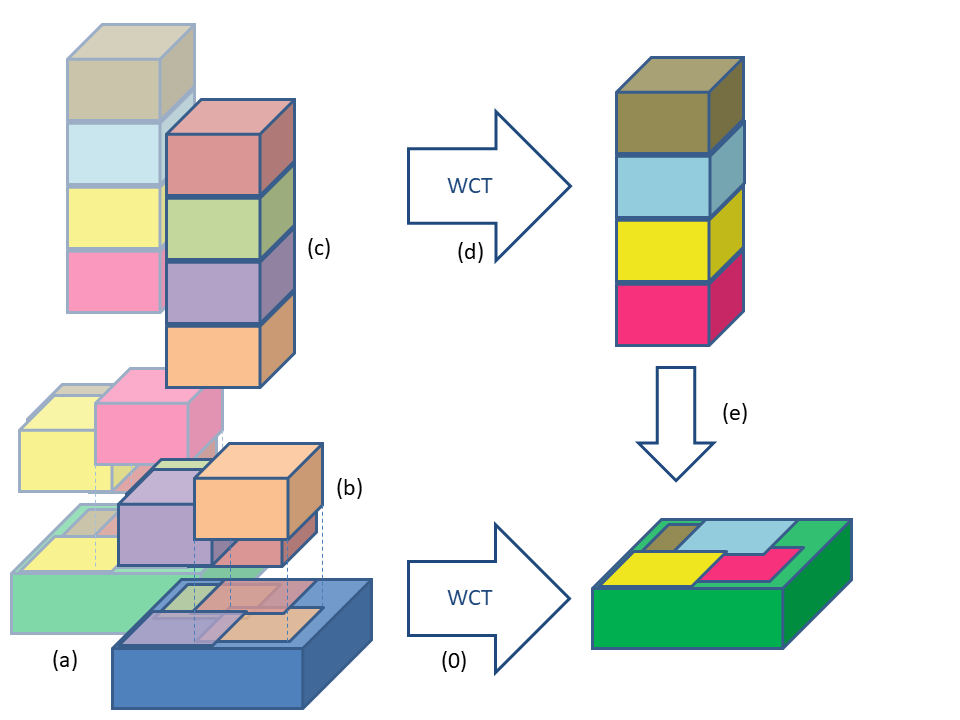
\includegraphics[width=0.6\linewidth]{boost_fig.png}
	\caption{Boost main steps. (0) is the ordinary WCT on $f_c$ and $f_s$, (a) is regions selection, (b) is region slicing, in (c) the regions are stacked, in (d) WCT is performed on the stacked regions with 512 channels, finally in (e) the boosted regions are blended into $f_{cs}$.}
	\label{fig:boost}
\end{figure}

Before refining the boost method to its final form we had tried to replace the original WCT altogether in architectures 1,2 and 3, such that \textbf{only} efficient SVD calls are conducted. Doing so, regions were not chosen, instead, the features were perfectly split into non overlapping sections. These were stacked, then came WCT, after which the sections were unstacked. The major drawback of that method is that these sections are treated as independent channels in the WCT, so clear border artifacts could be seen between them after the reconstruction. 



\subsection{Merge}
\label{merge_methods_lbl}
In their paper \cite{bib11}, Li et al describe an interpolation technique to generate texture from two input style images. According to their method, which we shall refer to as \textit{Original-Merge}, at each pipeline level two WCT calls are conducted: $f_{cs_1} = WCT(x, f_{s_1}), f_{cs_2} = WCT(x, f_{s_2})$ where $x$ is the content features output by the level encoder. The results are then interpolated with $f_{cs} = \beta f_{cs_1} + (1-\beta)f_{cs_2}$. After the interpolation, $f_{cs}$ is reconstructed as usual using the level decoder.\\

In this section we researched other merging techniques to merge two style with a \textbf{single} WCT call for each pipeline level. We present the following three techniques:

\begin{itemize}
	\item \textbf{Level Merge}: Let $P_1, \dots, P_k$ be the pipeline level functions. According to this notation, in Figure ~\ref{fig:full-pipeline} the output is a product of:
	\begin{equation*}
	I_{out} = P_5 ( P_4 ( P_3 ( P_2 ( P_1 (c,s),s) ,s),s), s)
	\end{equation*}
	To \textit{Level Merge} transfer content $c$ with style images $s_1$ and $s_2$ do the following:
	\begin{equation*}
	I_{out} = P_5 ( P_4 ( P_3 ( P_2 ( P_1 (c, s_1), s_2), s_1), s_2), s_1)
	\end{equation*}
	This method simply alternates the transferred style at each progression through the pipeline levels. In Level-Merge, the WCT procedure is called once per level, which makes it more computationally efficient than Original-Merge. Since in each level it calls for the encoder twice, the WCT once, and the decoder once, it has the same computational load of regular UST with one style image. As a side note, the $\beta$ parameter that controls the relative weight of each style cannot be used in this technique.
	 
	\item \textbf{Channel Merge}: Let $s_1, s_2$ be the input pair of styles, and let $c'$ be the content input to the $j$-th pipeline level. Under Channel Merge, we extract features for all three: $f_{s_1} = E_j(s_1), f_{s_2} = E_j(s_2), f_{c'} = E_j(c')$. Then, we split $f_{s_1}$ and $f_{s_2}$ for $d$ splits across the channel dimension to get $f_{s_1} = \begin{bmatrix} f_{s_1}^1 \\ \vdots \\ f_{s_1}^d\end{bmatrix}$ and $f_{s_2} = \begin{bmatrix} f_{s_2}^1 \\ \vdots \\ f_{s_2}^d\end{bmatrix}$. Then, create synthetic $\tilde{f_{s}}$ by alternatively stacking splits from $f_{s_1}$ and $f_{s_2}$. In our implementation we set  $d=4$, for which $\tilde{f_{s}} = \begin{bmatrix} f_{s_1}^1 \\  f_{s_2}^2 \\  f_{s_1}^3 \\ f_{s_2}^4\end{bmatrix}$. After that, the level output is achieved by $f_{c',s_1,s_2} = WCT(f_{c'}, \tilde{f_{s}})$, and then $c'' = D_j(f_{c',s_1,s_2})$. In Channel Merge, in each pipeline level, still a single WCT call is conducted, but three feature extractions are made, making it slightly more computationally heavy than the Level Merge method. A limitation to this technique is the necessity for the pair of style to have same dimensions, this can be achieved simply by resizing the style inputs. In this technique the $\beta$ parameter cannot be used as well.
	
	\item \textbf{Interpolate-Style Merge}: As described above, Original Merge conducts \textbf{two} WCT calls in each pipeline level and interpolates their results, before feeding it to the level decoder. Relating to this, in Interpolate-Style Merge, the extracted features of both styles are interpolated \textbf{before} the WCT call, which operates on the features of the content and the interpolated features of both styles together. Formally, to calculate $j$-th pipeline level output, $c_j$, do:
	\begin{enumerate}
		\item Input $c_{j-1}, s_1, s_2$
		\item Extract features: $f_{c_{j-1}} = E_j(c_{j-1})$, $f_{s_1} = E_j(f_{s_1})$, $f_{s_2} = E_j(f_{s_2})$
		\item Interpolate style features: $\tilde{f_{s}} = \beta\cdot f_{s_1} + (1-\beta)\cdot f_{s_2}$
		\item Run WCT: $f_{cs} = WCT(c_{j-1}, \tilde{f_{s}})$
		\item Output decoded $f_{cs}$: $c_j = D_j(f_{cs})$
	\end{enumerate}
	In this method too, in each pipeline level, still a single WCT call is conducted, and three feature extractions are made, making it slightly more computationally heavy than the Level Merge method. The same limitation from Channel Merge applies to this technique as well, is the necessary for the pair of style to have same dimensions, which is done, again, by resizing the style inputs. Unlike the other techniques proposed above, this technique can harness the functionality of the $\beta$ parameter to give weights to the styles while merging.
\end{itemize}
These three methods are implemented in the function \texttt{merge\_function} in file \texttt{utils.py}. Different merging methods are available at the \texttt{universal\_style\_transfer.py} by setting argument \texttt{--merge-method} to either 1,2,3,4. 
%show an improved algorithm which merges two style images bu using WCT algorithm which based on singular value decomposition (SVD). Here, we both implement the original merge algorithm as proposed in \cite{bib11} as well as introduce three additional efficient methods based on the use WCT.
	
	\section{Experiments}
	\label{experiments_lbl}
	%%%%%  Decoder %%%%%
\subsection{Reconstruction Quality Evaluation}

Our implementation of the Universal Style Transfer is adapted to use two different sets of encoder-decoder models: the models we trained according to section \ref{subsec:Models} (our), and the models offered to download by Li et al in their GitHub (reference). This means that we can test \textbf{our implementation} of the UST algorithm with both sets of models. In this section we want to evaluate our models in comparison to the references in terms of image reconstruction, in order to asses the quality of our models training.

\subsubsection{Quantative Reconstruction Loss}
As section \ref{subsec:Models} explains, the models are trained for image reconstruction. Passing an input image through the encoder-decoder models will output a reconstructed image, featuring some distortion. A better trained model will output images which feature smaller distortion. In order to quantify the reconstruction distortion induced by our trained models, in comparison to that of the reference models, we encode and then decode 1k content images from the COCO dataset with each of the 5 encoder-decoder pairs, and measure the pixel MSE and feature MSE (as depicted in equation \ref{eq:loss} and elaborated in \cite{bib22, bib17}). The pixel MSE measures the pixel mean square error between the reconstructed image, $\hat{x}$, and the original one, $x$, i.e. $MSE(x - \hat{x})$. The feature MSE measures the error between the deep features of the reconstructed image and the original one. It is measured by encoding $x$ and $\hat{x}$ and calculating $MSE(E(x)-E(\hat{x}))$. Table ~\ref{Tab:loss} displays the pixel loss (feature loss) per model, which is defined to be the average pixel MSE (feature MSE) over all 1k images.
 
% ecoder-decoder table %

\begin{center}
	\captionof{table}{Pixel and Feature Loss Per Model\label{Tab:loss}}
	\centering
	\begin{tabular}{ |>{\centering}p{2.5cm}||>{\centering}p{2.5cm}|>{\centering}p{2.5cm}|>{\centering}p{2.5cm}|>{\centering}p{2.5cm}| }
		\hline
		\multicolumn{5}{|c|}{\hspace{1.4cm} Pixel loss[$1\mathrm{e}{-4}$] \hspace{3cm}$\mid$ \hspace{1cm} Feature loss[$1\mathrm{e}{-2}$]} \\
		\hline
		architecture &Reference &Our &Reference &Our \tabularnewline
		\hline
		1 &$8.16$  &$784.42$   &$2.09$ &$0.71$\tabularnewline
		\hline
		2 &$2.27$  &$791.08$   &$1.24$ &$15.22$\tabularnewline
		\hline
		3 &$7.71$  &$866.33$   &$15.87$ &$85.44$\tabularnewline
		\hline
		4 &$27.76$  &$812.24$   &$24.48$ &$219.65$\tabularnewline
		\hline
		5 &$105.69$  &$798.14$   &$104.95$ & $39.67$\tabularnewline
		\hline
	\end{tabular}\\
\end{center}

From table ~\ref{Tab:loss} it is visible that in terms of pixel loss, the reconstruction done by the reference models is at least an order of magnitude better than of our models, sometimes two. It is also visible that the reference pixel loss generally increases as the architecture gets deeper, while ours is relatively constant. In the reference models, the pixel loss and feature loss show similar traits, which reassures $\lambda=1$ while training. In our models, on the other hand, the pixel loss and feature loss seem independent which may indicate the models have yet to fully converge. The impression from this data is that the models we trained perform worse than their reference counterparts.

%%%%%%%%%%%%%%%%%%%%%%%%%%%%%%%%%%%%%%%%%%
%%% reconstruction comparison %%%
%%%%%%%%%%%%%%%%%%%%%%%%%%%%%%%%%%%%%%%%%%
\subsubsection{Qualitative Reconstruction Loss}
To demonstrate the image reconstruction performance of our trained models, we choose 5 different images and feed them as input to both our encoder-decoder architectures, and the references. The results, as presented in figure ~\ref{fig:reconstruction}, visualize the image reconstruction quality of our models in comparison to that of the references. Column (a) consists of the original images, (b) presents the reconstruction results for encoder-decoder architecture \#1, columns (c)-(f) present the same for architectures 2-5 as depicted in \ref{subsec:Models}, and column (g) presents the reconstruction result done by the reference encoder-decoder architecture \#5. 

%%%%%%%%%%%%%%%%%%%%%%%%%%%%%% Reconstrucion images %%%%%%%%%%%%%%%%%%%%%%%%%%%%%%%%%%
\begin{figure}[H]
	% first line
	\centering
	\begin{subfigure}[b]{0.13\linewidth}
		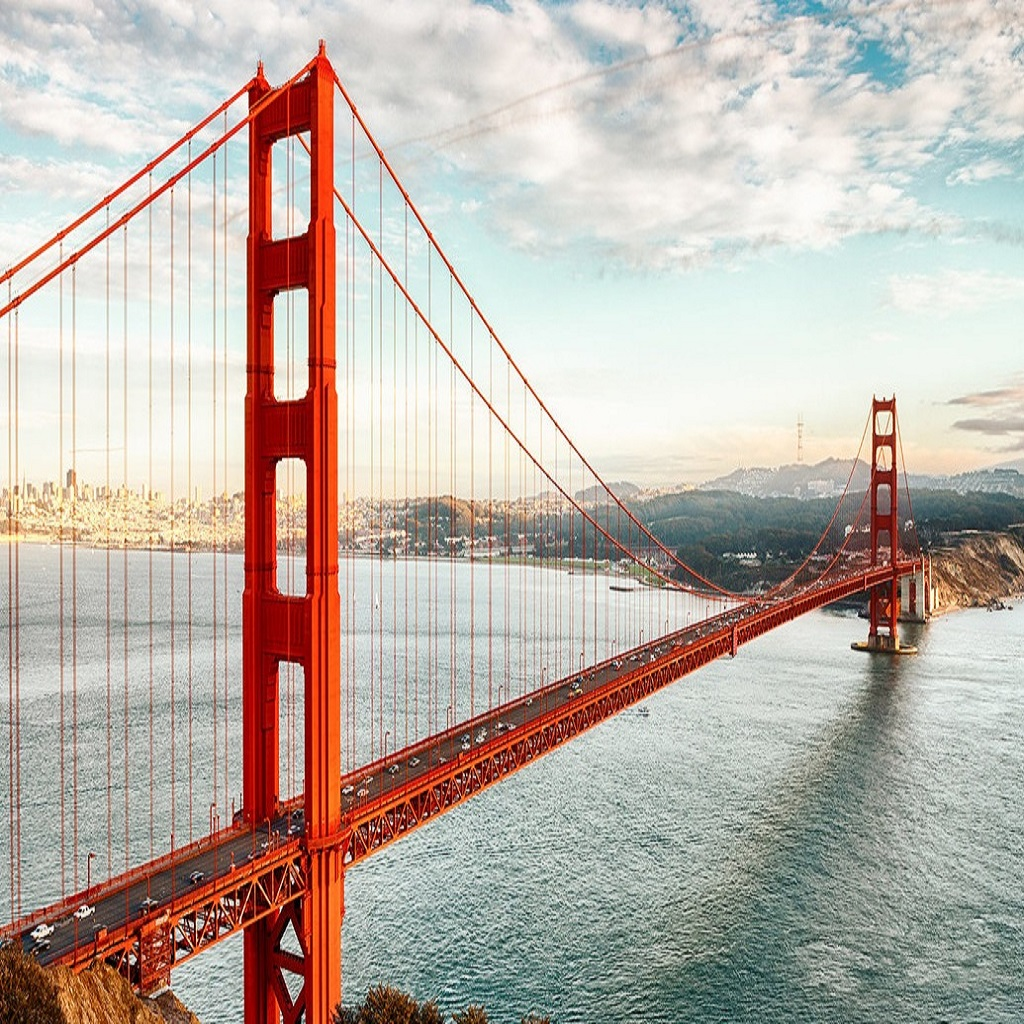
\includegraphics[width=\linewidth]{bridge_sq.jpg} % original num.1	
	\end{subfigure}
	\begin{subfigure}[b]{0.13\linewidth}
		\includegraphics[width=\linewidth]{reconst_exper/dec_bridge_my_1_test.jpg} % our reconstruction arc1 num.1	
	\end{subfigure}
	\begin{subfigure}[b]{0.13\linewidth}
		\includegraphics[width=\linewidth]{reconst_exper/dec_bridge_my_2_test.jpg} % our reconstruction arc2 num.1	
	\end{subfigure}
	\begin{subfigure}[b]{0.13\linewidth}
		\includegraphics[width=\linewidth]{reconst_exper/dec_bridge_my_3_test.jpg} % our reconstruction arc3 num.1	
	\end{subfigure}
	\begin{subfigure}[b]{0.13\linewidth}
		\includegraphics[width=\linewidth]{reconst_exper/dec_bridge_my_4_test.jpg} % our reconstruction arc4 num.1	
	\end{subfigure}
	\begin{subfigure}[b]{0.13\linewidth}
		\includegraphics[width=\linewidth]{reconst_exper/dec_bridge_my_5_test.jpg} % our reconstruction arc5 num.1	
	\end{subfigure}
	\begin{subfigure}[b]{0.13\linewidth}
		\includegraphics[width=\linewidth]{reconst_exper/dec_bridge_ref_5_test.jpg} % their reconstruction arc5 num.1	
	\end{subfigure}
	% second line
	\centering
	\begin{subfigure}[b]{0.13\linewidth}
		\includegraphics[width=\linewidth]{giraffe_sq.jpg} % original num.1	
	\end{subfigure}
	\begin{subfigure}[b]{0.13\linewidth}
		\includegraphics[width=\linewidth]{reconst_exper/dec_giraffe_my_1_test.jpg} % our reconstruction arc1 num.1	
	\end{subfigure}
	\begin{subfigure}[b]{0.13\linewidth}
		\includegraphics[width=\linewidth]{reconst_exper/dec_giraffe_my_2_test.jpg} % our reconstruction arc2 num.1	
	\end{subfigure}
	\begin{subfigure}[b]{0.13\linewidth}
		\includegraphics[width=\linewidth]{reconst_exper/dec_giraffe_my_3_test.jpg} % our reconstruction arc3 num.1	
	\end{subfigure}
	\begin{subfigure}[b]{0.13\linewidth}
		\includegraphics[width=\linewidth]{reconst_exper/dec_giraffe_my_4_test.jpg} % our reconstruction arc4 num.1	
	\end{subfigure}
	\begin{subfigure}[b]{0.13\linewidth}
		\includegraphics[width=\linewidth]{reconst_exper/dec_giraffe_my_5_test.jpg} % our reconstruction arc5 num.1	
	\end{subfigure}
	\begin{subfigure}[b]{0.13\linewidth}
		\includegraphics[width=\linewidth]{reconst_exper/dec_giraffe_ref_5_test.jpg} % their reconstruction arc5 num.1	
	\end{subfigure}
	% third line
	\centering
	\begin{subfigure}[b]{0.13\linewidth}
		\includegraphics[width=\linewidth]{in1_sq.jpg} % original num.1	
	\end{subfigure}
	\begin{subfigure}[b]{0.13\linewidth}
		\includegraphics[width=\linewidth]{reconst_exper/dec_in1_my_1_test.jpg} % our reconstruction arc1 num.1	
	\end{subfigure}
	\begin{subfigure}[b]{0.13\linewidth}
		\includegraphics[width=\linewidth]{reconst_exper/dec_in1_my_2_test.jpg} % our reconstruction arc2 num.1	
	\end{subfigure}
	\begin{subfigure}[b]{0.13\linewidth}
		\includegraphics[width=\linewidth]{reconst_exper/dec_in1_my_3_test.jpg} % our reconstruction arc3 num.1	
	\end{subfigure}
	\begin{subfigure}[b]{0.13\linewidth}
		\includegraphics[width=\linewidth]{reconst_exper/dec_in1_my_4_test.jpg} % our reconstruction arc4 num.1	
	\end{subfigure}
	\begin{subfigure}[b]{0.13\linewidth}
		\includegraphics[width=\linewidth]{reconst_exper/dec_in1_my_5_test.jpg} % our reconstruction arc5 num.1	
	\end{subfigure}
	\begin{subfigure}[b]{0.13\linewidth}
		\includegraphics[width=\linewidth]{reconst_exper/dec_in1_ref_5_test.jpg} % their reconstruction arc5 num.1	
	\end{subfigure}
	%fourth line
	\centering
	\begin{subfigure}[b]{0.13\linewidth}
		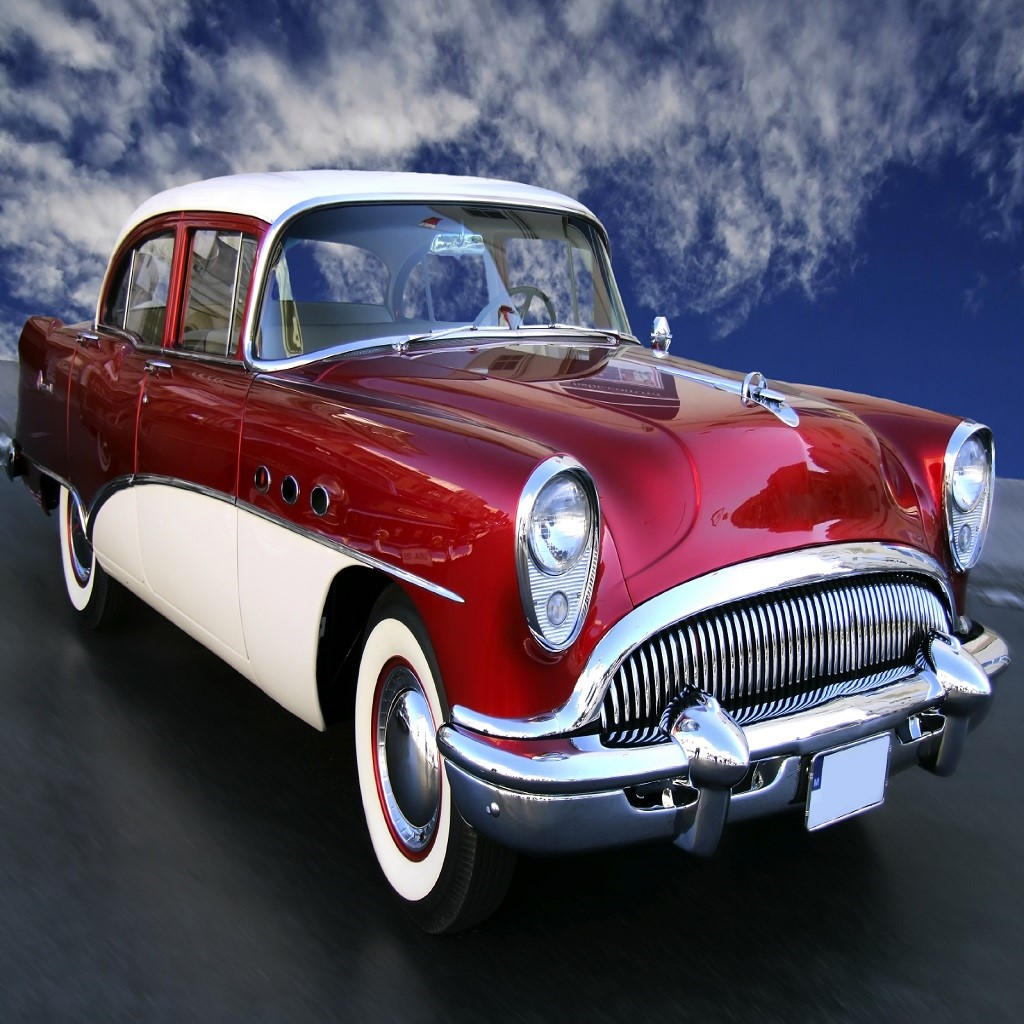
\includegraphics[width=\linewidth]{car_sq.jpg} % original num.1	
	\end{subfigure}
	\begin{subfigure}[b]{0.13\linewidth}
		\includegraphics[width=\linewidth]{reconst_exper/dec_in2_my_1_test.jpg} % our reconstruction arc1 num.1	
	\end{subfigure}
	\begin{subfigure}[b]{0.13\linewidth}
		\includegraphics[width=\linewidth]{reconst_exper/dec_in2_my_2_test.jpg} % our reconstruction arc2 num.1	
	\end{subfigure}
	\begin{subfigure}[b]{0.13\linewidth}
		\includegraphics[width=\linewidth]{reconst_exper/dec_in2_my_3_test.jpg} % our reconstruction arc3 num.1	
	\end{subfigure}
	\begin{subfigure}[b]{0.13\linewidth}
		\includegraphics[width=\linewidth]{reconst_exper/dec_in2_my_4_test.jpg} % our reconstruction arc4 num.1	
	\end{subfigure}
	\begin{subfigure}[b]{0.13\linewidth}
		\includegraphics[width=\linewidth]{reconst_exper/dec_in2_my_5_test.jpg} % our reconstruction arc5 num.1	
	\end{subfigure}
	\begin{subfigure}[b]{0.13\linewidth}
		\includegraphics[width=\linewidth]{reconst_exper/dec_in2_ref_5_test.jpg} % their reconstruction arc5 num.1	
	\end{subfigure}
	% fifth line
	\centering
	\begin{subfigure}[b]{0.13\linewidth}
		\includegraphics[width=\linewidth]{room_sq.jpg} % original num.5
		\caption{Original}
	\end{subfigure}
	\begin{subfigure}[b]{0.13\linewidth}
		\includegraphics[width=\linewidth]{reconst_exper/dec_room_my_1_test.jpg} % our reconstruction num.5
		\caption{Ours arc1}
	\end{subfigure}
	\begin{subfigure}[b]{0.13\linewidth}
		\includegraphics[width=\linewidth]{reconst_exper/dec_room_my_2_test.jpg} % our reconstruction num.5
		\caption{Ours arc2}
	\end{subfigure}
	\begin{subfigure}[b]{0.13\linewidth}
		\includegraphics[width=\linewidth]{reconst_exper/dec_room_my_3_test.jpg} % our reconstruction num.5
		\caption{Ours arc3}
	\end{subfigure}
	\begin{subfigure}[b]{0.13\linewidth}
		\includegraphics[width=\linewidth]{reconst_exper/dec_room_my_4_test.jpg} % our reconstruction num.5
		\caption{Ours arc4}
	\end{subfigure}
	\begin{subfigure}[b]{0.13\linewidth}
		\includegraphics[width=\linewidth]{reconst_exper/dec_room_my_5_test.jpg} % our reconstruction num.5
		\caption{Ours arc5}
	\end{subfigure}
	\begin{subfigure}[b]{0.13\linewidth}
		\includegraphics[width=\linewidth]{reconst_exper/dec_room_ref_5_test.jpg} % their reconstruction arc5 num.1
		\caption{Ref arc5}	
	\end{subfigure}
	\caption{Image Reconstruction in different architectures}
	\label{fig:reconstruction}
\end{figure}

From Figure ~\ref{fig:reconstruction} it can be seen that our architectures \#1-4 conserve the original image's color to some degree. Architecture \#5, unlike them, only preserves a fraction of the color tones originally available in the input - mostly some of the reds. Additionally, the deeper the architecture is, the more details are lost in the reconstruction process. Another problem is image regions going gray, and losing their contrast, such as the shade of the car in the fourth row or the blue walls in the fifth. Keeping in mind the trade-off between pipeline depth and image distortion, in order to get the best results possible from the models trained by us, we choose to shorten our pipeline such that it would consist of the four last pipeline levels from ~\ref{fig:style_transfer}. In this way we expect our pipeline to produce good reconstruction quality as well as use deep enough features while transferring style. This means we leave architecture \#5 unused when transferring style using our trained models.\\
These visual results show that our models are not sufficiently trained. The main difficulty in training these models was a lack of compute power. The models, based on VGG-19 are relatively large and converge very slowly towards optimality. We strongly believe that given more powerful resources we could have trained better performing decoders.\\
\textcolor{red}{Consider making an experiment showing reconstruction through the pipeline 4321, next to style transfer or just next to the reference (justification for choosing 4321 as our pipeline)}
  
%%%%%%%%%%%%%%%%%%%%%%%%%%%%
%%%%%%%%%%%%%%%%%%%%%%%%%%%%
% style transfer images %
%%%%%%%%%%%%%%%%%%%%%%%%%%%%
%%%%%%%%%%%%%%%%%%%%%%%%%%%%

\subsection{Style Transfer Experimental Results}
This section displays the results of our implementation of UST\cite{bib11}. Unlike the previous section where the images only went through reconstruction, this time we run the entire algorithm implementation, including the WCT at the bottleneck of the model-decoder pipeline levels. Due to reasons explained above, when using our trained models the pipeline consists of architectures \#1-4, while it consists of architectures \#1-5 when our implementation uses the reference models. In figure ~\ref{fig:style_transfer} we show several examples of style transferral using our implementation with both sets of models. Column (a) shows the input content images, column (b) shows the input style images, column (c) shows the results computed using the reference models and (d) using ours.\\

\begin{figure}[H]
	% first line
	\centering
	\begin{subfigure}[b]{0.225\linewidth}
		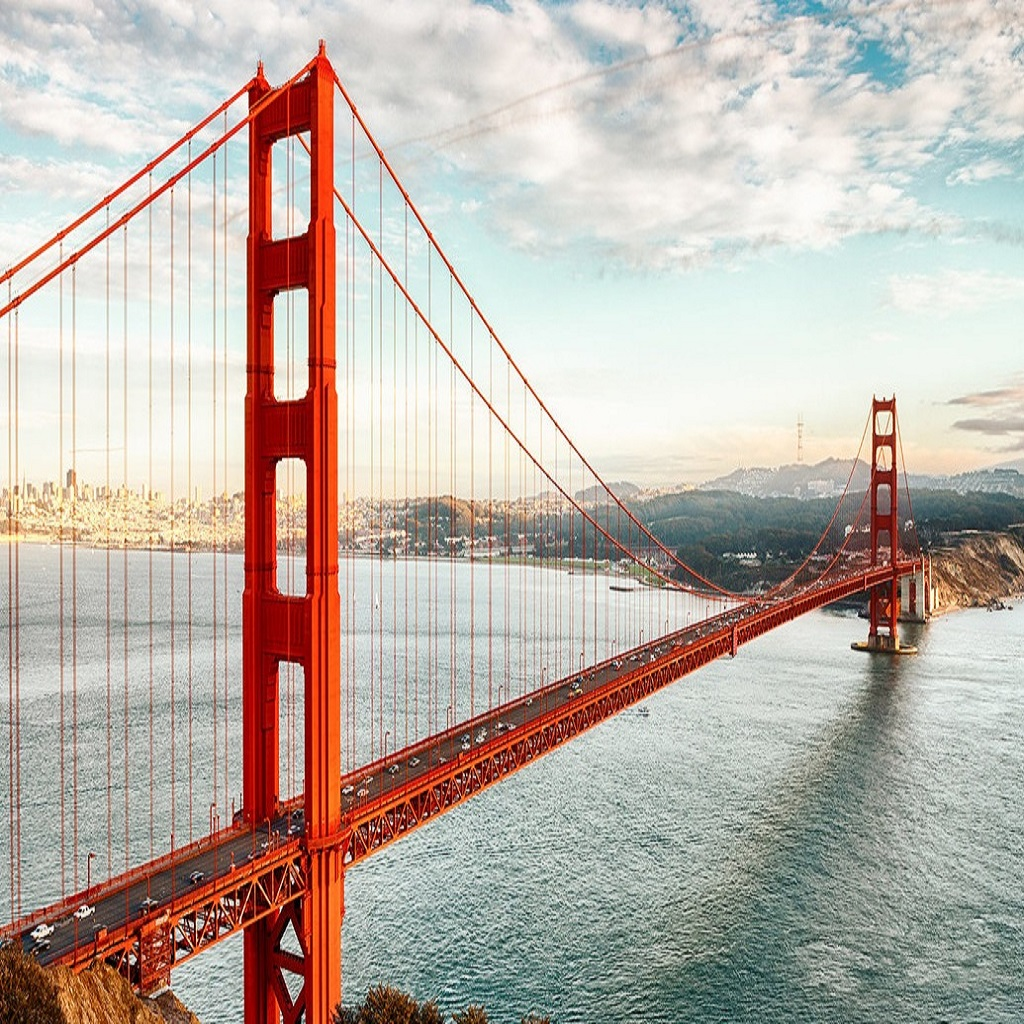
\includegraphics[width=\linewidth]{bridge_sq.jpg} % content img num.1
	\end{subfigure}
	\begin{subfigure}[b]{0.225\linewidth}
		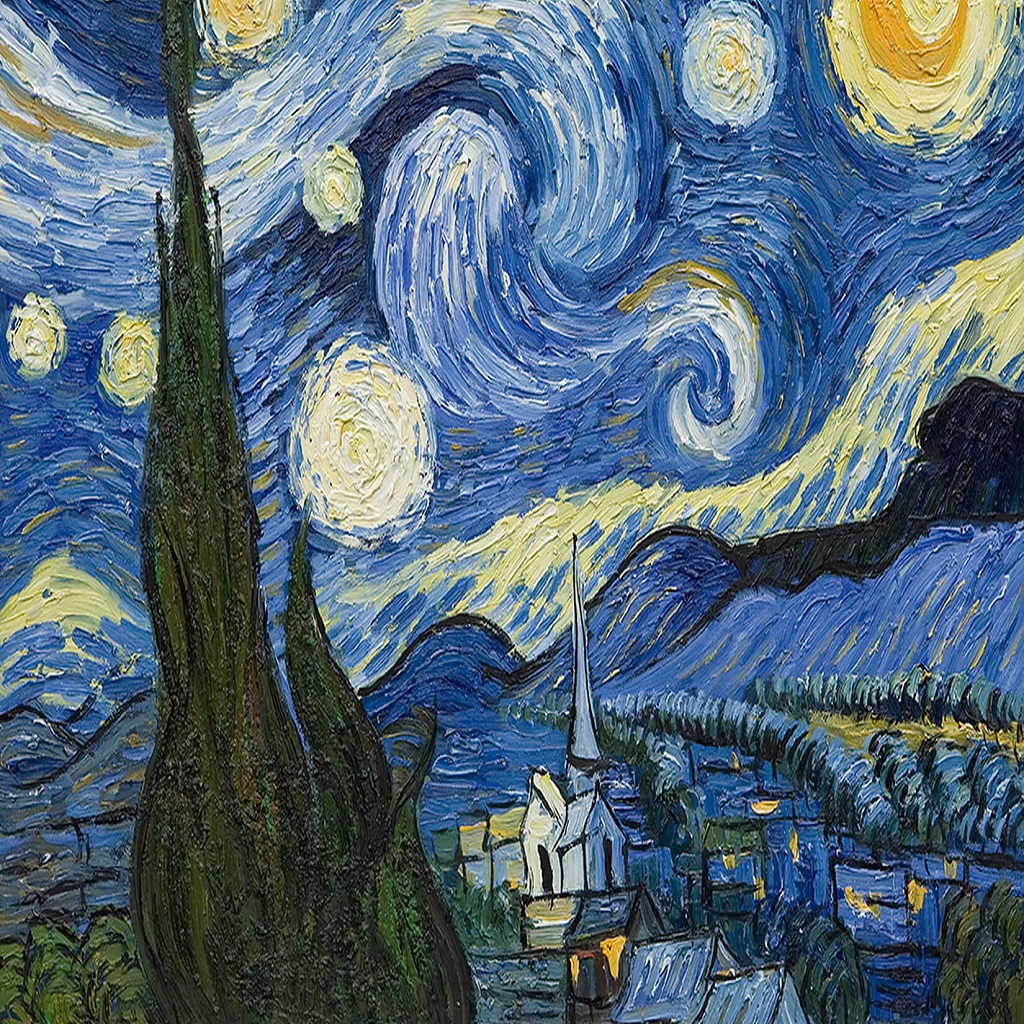
\includegraphics[width=\linewidth]{starry_sq.jpg} % style img num.1	
	\end{subfigure}
	\begin{subfigure}[b]{0.225\linewidth}
		\includegraphics[width=\linewidth]{transfer_examples/transfer_bridge_starry_08_ref.jpg} % theirs reconstruction num.1	
	\end{subfigure}
	\begin{subfigure}[b]{0.225\linewidth}
		\includegraphics[width=\linewidth]{transfer_examples/transfer_bridge_starry_08_our.jpg} % ours reconstruction num.1	
	\end{subfigure}
	% second line
	\centering
	\begin{subfigure}[b]{0.225\linewidth}
		\includegraphics[width=\linewidth]{giraffe_sq.jpg} % content img num.2
	\end{subfigure}
	\begin{subfigure}[b]{0.225\linewidth}
		\includegraphics[width=\linewidth]{st1_sq.jpg} % style img num.2
	\end{subfigure}
	\begin{subfigure}[b]{0.225\linewidth}
		\includegraphics[width=\linewidth]{transfer_examples/transfer_giraffe_st1_08_ref.jpg} % theirs reconstruction num.2
	\end{subfigure}
	\begin{subfigure}[b]{0.225\linewidth}
		\includegraphics[width=\linewidth]{transfer_examples/transfer_giraffe_st1_08_our.jpg} % ours reconstruction num.2
	\end{subfigure}
	% third line
	\centering
	\begin{subfigure}[b]{0.225\linewidth}
		\includegraphics[width=\linewidth]{in1_sq.jpg} % content img num.3
	\end{subfigure}
	\begin{subfigure}[b]{0.225\linewidth}
		\includegraphics[width=\linewidth]{tiger_sq.jpg} % style img num.3
	\end{subfigure}
	\begin{subfigure}[b]{0.225\linewidth}
		\includegraphics[width=\linewidth]{transfer_examples/transfer_in1_tiger_08_ref.jpg} % theirs reconstruction num.3
	\end{subfigure}
	\begin{subfigure}[b]{0.225\linewidth}
		\includegraphics[width=\linewidth]{transfer_examples/transfer_in1_tiger_08_our.jpg} % ours reconstruction num.3
	\end{subfigure}
	% fourth line
	\centering
	\begin{subfigure}[b]{0.225\linewidth}
		\includegraphics[width=\linewidth]{nyc_sq.jpg} % content img num.4
	\end{subfigure}
	\begin{subfigure}[b]{0.225\linewidth}
		\includegraphics[width=\linewidth]{graffiti_sq.jpg} % style img num.4
	\end{subfigure}
	\begin{subfigure}[b]{0.225\linewidth}
		\includegraphics[width=\linewidth]{transfer_examples/transfer_nyc_graffiti_08_ref.jpg} % theirs reconstruction num.4
	\end{subfigure}
	\begin{subfigure}[b]{0.225\linewidth}
		\includegraphics[width=\linewidth]{transfer_examples/transfer_nyc_graffiti_08_our.jpg} % ours reconstruction num.4
	\end{subfigure}
	% fifth line
	\centering
	\begin{subfigure}[b]{0.225\linewidth}
		\includegraphics[width=\linewidth]{room_sq.jpg} % content img num.5
		\caption{Content}
	\end{subfigure}
	\begin{subfigure}[b]{0.225\linewidth}
		\includegraphics[width=\linewidth]{st2_sq.jpg} % style img num.5
		\caption{Style}
	\end{subfigure}
	\begin{subfigure}[b]{0.225\linewidth}
		\includegraphics[width=\linewidth]{transfer_examples/transfer_room_paint_08_ref.jpg} % theirs reconstruction num.5
		\caption{Reference Models}
	\end{subfigure}
	\begin{subfigure}[b]{0.225\linewidth}
		\includegraphics[width=\linewidth]{transfer_examples/transfer_room_paint_08_our.jpg} % ours reconstruction num.5
		\caption{Our Models}
	\end{subfigure}
	\caption{Results of our UST implementation, using two sets of models, with $\alpha=0.5$}
	\label{fig:style_transfer}
\end{figure}

It is seen in the results displayed in Figure ~\ref{fig:style_transfer} (c)+(d) that our implementation of the UST algorithm works and that given a pair of content and style images it outputs a new image that resembles the former in its content and the latter in its artistic style. As earlier mentioned the results produced by our models suffer from artifacts of gray areas originating in the reconstruction distortion. Generally column (d) shows results less pleasing than those in column (c) but clearly answers the definition of Style Transfer. \\

%%%%%%%%%%%%%%%%%%%%%%%%%%%%
%%%%%%%%%%%%%%%%%%%%%%%%%%%%
% Boost %
%%%%%%%%%%%%%%%%%%%%%%%%%%%%
%%%%%%%%%%%%%%%%%%%%%%%%%%%%
\subsubsection{Stylization Boosting}
This section presents the results of the innovative \textit{boost} step we introduced to the UST algorithm. Figures ~\ref{fig:Boost1} and ~\ref{fig:Boost2} show examples of boosting the UST. It is noticeable that boosted regions contain more finely detailed style and color than their non-boosted counterparts. The details in the boosted regions are more intense and colorful, and the boosting step achieves this without harming the original content of these regions. As the results show, our boosting step could be adapted to the UST algorithm to achieve visually better results. In order to show the true potential of the boost step, these results were produced with our implementation of the UST using the reference models.

\begin{figure}[H]
	% first line
	\centering
	\begin{subfigure}[b]{0.4\linewidth}
		\includegraphics[width=\linewidth]{car_sq.jpg} % content img num.1
		%\caption{Content}
	\end{subfigure}
	\begin{subfigure}[b]{0.4\linewidth}
		\includegraphics[width=\linewidth]{st2_sq.jpg} % style img num.1
		%\caption{Style}
	\end{subfigure}
	%second line
	\begin{subfigure}[b]{0.4\linewidth}
		\includegraphics[width=\linewidth]{boost/boost_in2_st2_05_no.jpg} % regular UST num.1
		%\caption{Regular UST}
	\end{subfigure}
	\begin{subfigure}[b]{0.4\linewidth}
		\includegraphics[width=\linewidth]{boost/boost_in2_st2_05.jpg} % UST+boost num.1
		%\caption{Boost UST}
	\end{subfigure}
	\caption{First Boosting results comparing to original UST \cite{bib11}. Top left is the content image, top right is the style image, bottom left is the regular UST, bottom right is the UST+boost}
	\label{fig:Boost1}
\end{figure}
\begin{figure}[H]
	\centering
	\begin{subfigure}[b]{0.4\linewidth}
		\includegraphics[width=\linewidth]{room_sq.jpg} % content img num.1
		%\caption{Content}
	\end{subfigure}
	\begin{subfigure}[b]{0.4\linewidth}
		\includegraphics[width=\linewidth]{giraffe_sq.jpg} % style img num.1
		%\caption{Style}
	\end{subfigure}
	%second line
	\begin{subfigure}[b]{0.4\linewidth}
		\includegraphics[width=\linewidth]{boost/boost_room_giraffe_05_no.jpg} % regular UST num.1
		%\caption{Regular UST}
	\end{subfigure}
	\begin{subfigure}[b]{0.4\linewidth}
		\includegraphics[width=\linewidth]{boost/boost_room_giraffe_05.jpg} % UST+boost num.1
		%\caption{Boost UST}
	\end{subfigure}
	\caption{Second Boosting results comparing to original UST \cite{bib11}. Top left is the content image, top right is the style image, bottom left is the regular UST, bottom right is the UST+boost}
	\label{fig:Boost2}
\end{figure}

%%%%%%%%%%%%%%%%%%%%%%%% Merge  %%%%%%%%%%%%%%%%%%%%%%
\subsubsection{Two styles merging methods}
This section presents the results of our innovative \textit{Merging} techniques we introduced to the UST algorithm. Figure~\ref{fig:Merge} shows examples of merging two styles to one content using these three techniques in comparison to the original technique offered in \cite{bib11}. First thing noticeable is that all techniques perform Merge-UST with visually pleasing results. The Interpolate-Style Merge shown in column (e) features surprisingly similar results to Original-Merge, even though it uses one WCT call instead of two, making it computationally more efficient. As the results show, our innovative merging techniques could be adapted to the UST algorithm to achieve the same visually pleasing results with decreased computational complexity. In order to show the true potential the merging techniques, these results were produced with our implementation of the UST using the reference models.

\begin{figure}[H]
	% first line
	\centering
	\begin{subfigure}[b]{0.13\linewidth}
		\includegraphics[width=\linewidth]{bridge_sq.jpg} % content img num.1
	\end{subfigure}
	\begin{subfigure}[b]{0.13\linewidth}
		\includegraphics[width=\linewidth]{starry_sq.jpg} % style1 img num.1
	\end{subfigure}
	\begin{subfigure}[b]{0.13\linewidth}
		\includegraphics[width=\linewidth]{st2_sq.jpg} % style2 img num.1
	\end{subfigure}
	\begin{subfigure}[b]{0.13\linewidth}
		\includegraphics[width=\linewidth]{merge/merge_bridge_starry_st2_1.jpg} % orig merge num.1
	\end{subfigure}
	\begin{subfigure}[b]{0.13\linewidth}
		\includegraphics[width=\linewidth]{merge/merge_bridge_starry_st2_4.jpg} % merge1 num.1
	\end{subfigure}
	\begin{subfigure}[b]{0.13\linewidth}
		\includegraphics[width=\linewidth]{merge/merge_bridge_starry_st2_2.jpg} % merge2 num.1
	\end{subfigure}
	\begin{subfigure}[b]{0.13\linewidth}
		\includegraphics[width=\linewidth]{merge/merge_bridge_starry_st2_3.jpg} % merge3 num.1
	\end{subfigure}
	% second line
	\centering
	\begin{subfigure}[b]{0.13\linewidth}
		\includegraphics[width=\linewidth]{face_sq.jpg} % content img num.2
	\end{subfigure}
	\begin{subfigure}[b]{0.13\linewidth}
		\includegraphics[width=\linewidth]{brick_sq.jpg} % style1 img num.2
	\end{subfigure}
	\begin{subfigure}[b]{0.13\linewidth}
		\includegraphics[width=\linewidth]{graffiti_sq.jpg} % style2 img num.2
	\end{subfigure}
	\begin{subfigure}[b]{0.13\linewidth}
		\includegraphics[width=\linewidth]{merge/merge_face_brick_graffiti_1.jpg} % orig merge num.2
	\end{subfigure}
	\begin{subfigure}[b]{0.13\linewidth}
		\includegraphics[width=\linewidth]{merge/merge_face_brick_graffiti_4.jpg} % merge1 num.2
	\end{subfigure}
	\begin{subfigure}[b]{0.13\linewidth}
		\includegraphics[width=\linewidth]{merge/merge_face_brick_graffiti_2.jpg} % merge2 num.2
	\end{subfigure}
	\begin{subfigure}[b]{0.13\linewidth}
		\includegraphics[width=\linewidth]{merge/merge_face_brick_graffiti_3.jpg} % merge3 num.2
	\end{subfigure}
	% third line
	\centering
	\begin{subfigure}[b]{0.13\linewidth}
		\includegraphics[width=\linewidth]{in1_sq.jpg} % content img num.3
		\caption{Content \\ image}
	\end{subfigure}
	\begin{subfigure}[b]{0.13\linewidth}
		\includegraphics[width=\linewidth]{st1_sq.jpg} % style1 img num.3
		\caption{$1^{st}$ \\ Style}
	\end{subfigure}
	\begin{subfigure}[b]{0.13\linewidth}
		\includegraphics[width=\linewidth]{tiger_sq.jpg} % style2 img num.3
		\caption{$2^{nd}$ \\ Style}
	\end{subfigure}
	\begin{subfigure}[b]{0.13\linewidth}
		\includegraphics[width=\linewidth]{merge/merge_in1_st1_tiger_1.jpg} % orig merge num.3
		\caption{Original Merge}
	\end{subfigure}
	\begin{subfigure}[b]{0.13\linewidth}
		\includegraphics[width=\linewidth]{merge/merge_in1_st1_tiger_4.jpg} % merge1 num.3
		\caption{Interp. Merge}
	\end{subfigure}
	\begin{subfigure}[b]{0.13\linewidth}
		\includegraphics[width=\linewidth]{merge/merge_in1_st1_tiger_2.jpg} % merge2 num.3
		\caption{Channel Merge}
	\end{subfigure}
	\begin{subfigure}[b]{0.13\linewidth}
		\includegraphics[width=\linewidth]{merge/merge_in1_st1_tiger_3.jpg} % merge3 num.3
		\caption{Level Merge}
	\end{subfigure}
		\caption{Results using different stylization methods.}
		\label{fig:Merge}
\end{figure}
%%%%%%%%%%%%%%%%%%%%%%%%%%%%


\textbf{Style-Merging Methods Efficiency}:\\
To quantify the runtime efficiency of the our new merging techniques in comparison to Original-Merge, we measured the runtime of our Merge-UST in all different techniques, and display the results in Table~\ref{Tab:merge}. The algorithm ran on $1024\times 1024$ RGB images. We averaged the results of 10 experiments per technique. The time was measured by the \texttt{time} bash command, and the displayed results are of the "User" runtime.
%Efficiency table%
\begin{center}
	\captionof{table}{UST merge runtime of different techniques\label{Tab:merge}}
	\begin{tabular}{||c| |c| |c| |c| |c||} 
		\hline
		\space & Original & Interpolation & Channel & Level \\ [0.5ex] 
		\hline\hline
		Time[sec] & 7.42 & 6.94 & 6.80 & 6.17\\ 
		\hline
	\end{tabular}
\end{center}

Table~\ref{Tab:merge} shows what was predicted in section~\ref{merge_methods_lbl}, i.e. all three techniques work faster than the Original-Merge, where Level-Merge is the fastest, working at regular UST speed, Interpolate-Style-Merge and Channel-Merge are roughly the same, and both save approximately $500ms$ comparing to Original-Merge. In this aspect the new techniques are superior.

%%%%%%%%%%%%%%%%%%%%%%%% Texture synthesis  %%%%%%%%%%%%%%%%%%%%%%
\subsubsection{Texture synthesis}
Another application for UST is Universal Texture Synthesis. As described in section~\ref{subsec:texture}, running the UST algorithm with random noise content input can serve as a texture generator, transferring the artistic style onto the noise. In Figure~\ref{fig:texture} we show examples of how our implementation of the UST can generate textures. The content inputs are uniform random noise. By the criterion set in section~\ref{subsec:texture}, it is noticeable that the generated textures differ from the originals, but we still consider them as visually pleasing.

\begin{figure}[H]
	% first line
	\centering
	\begin{subfigure}[b]{0.4\linewidth}
		\includegraphics[width=\linewidth]{brick_sq.jpg} %style img num.1
	\end{subfigure}
	\begin{subfigure}[b]{0.4\linewidth}
		\includegraphics[width=\linewidth]{texture_synth/brick_tex.jpg} % stylization img num.1
	\end{subfigure}
	% second line
	\centering
	\begin{subfigure}[b]{0.4\linewidth}
		\includegraphics[width=\linewidth]{cubism2_sq.jpg} %style img num.2
		\caption{Style}
	\end{subfigure}
	\begin{subfigure}[b]{0.4\linewidth}
		\includegraphics[width=\linewidth]{texture_synth/cubism2_tex.jpg} % stylization img num.2
		\caption{Our UST}
	\end{subfigure}
	\caption{UST Synthesized results.}
	\label{fig:texture}
\end{figure}
	
	\section{Conclusions}
	\label{conclusions_lbl}
	In this project we implemented the Universal Style Transfer algorithm as a lightweight PyTorch tool which is ready to be used by users. Additionally, since \textcolor{red}{describe somewhere} this tool supports hot replacement of its encoder-decoder models, researchers may use our tool to test the UST algorithm with different sets of models. Furthermore, our tool contains upgrades to the original algorithm in two aspects: Boost and Merge. The Boost step is an innovative procedure to enhance the style transfer effect on the result image, it has a practical application and produces better results. In the merging aspect, we offered three innovative techniques to perform style transfer with two style images, all of which are more time-efficient than the original technique in UST. In future research, it is possible to study extensions of our merging techniques that would allow for UST with more than a pair of style images. Additionally it is worthwhile to study the effect of multiple boost steps where we conducted one.

%training - more resources - or smaller models\\
%we implemented UST as a lightweight tool ready to use by users + available interface for switching models by replacing the ref\_models\_factory.py \\
%innovative new step for the UST algorithm: Boost, that can have practical applications. Learned that adding channels and downsizing h,w increases the style transfer effect without harming the content\\
%innovative new merging techniques which save runtime and feature results on par with the original technique. - Learned that the SVD is a major time consumer in the UST and reducing calls to SVD may reduce up to 7\% in the program runtime during merge.\\

%suggest ideas:\\
%formulate merging techniques for merging more than two styles.
%research the effect of multiple boost effects per pipeline level.


	%\section{References}
	\label{references_lbl}
	\input{references}
	
	\pagebreak
	\section{Appendix}
	\label{appendix_lbl}
	All code can be found also in our GitHub: \url{https://github.com/eyalw711/universal_style_transfer}
%\begin{itemize}
%\item \textbf{Main File}: \texttt{universal\_style\_transfer.py} \\	%\lstinputlisting[language=Python]{../universal_style_transfer.py}

%\item \textbf{Models File}:  \texttt{seq\_models.py} \\	%\lstinputlisting[language=Python]{../seq_models.py}

%\item \textbf{Models Utils File}:  \texttt{models\_utils.py} \\	%\lstinputlisting[language=Python]{../models_utils.py}

%\item \textbf{Utils File}:  \texttt{utils.py} \\	\lstinputlisting[language=Python]{../utils.py}

%\item \textbf{Reference Models Loader}:  \texttt{ref\_models\_factory.py} \\	%\lstinputlisting[language=Python]{../ref_models_factory.py}
%\end{itemize}

\end{document}
